\documentclass[11pt]{article}
\usepackage[a4paper,margin=24mm,headheight=15pt]{geometry}
\usepackage{fontspec}
\setmainfont{LiberationSerif-Regular.ttf}[Path=fonts/,BoldFont=LiberationSerif-Bold.ttf,ItalicFont=LiberationSerif-Italic.ttf,BoldItalicFont=LiberationSerif-BoldItalic.ttf]
\setsansfont{LiberationSans-Regular.ttf}[Path=fonts/,BoldFont=LiberationSans-Bold.ttf,ItalicFont=LiberationSans-Italic.ttf,BoldItalicFont=LiberationSans-BoldItalic.ttf]
\setmonofont{DejaVuSansMono.ttf}[Path=fonts/,Scale=0.83,BoldFont=DejaVuSansMono-Bold.ttf,ItalicFont=DejaVuSansMono-Oblique.ttf,BoldItalicFont=DejaVuSansMono-BoldOblique.ttf]
\usepackage{polyglossia}
\usepackage{amsmath,amssymb,booktabs,longtable,array,graphicx,xcolor}
\usepackage[font=small,labelfont=bf]{caption}
\usepackage{microtype}
\usepackage{placeins}
\usepackage{enumitem}
\setlist{nosep,leftmargin=*}
\usepackage[numbers,sort&compress]{natbib}
\usepackage[unicode,colorlinks=true,linkcolor=blue!45!black,citecolor=blue!45!black,urlcolor=blue!45!black]{hyperref}
\usepackage{xurl}
\usepackage{fancyhdr}
\pagestyle{fancy}\fancyhf{}\fancyhead[L]{\small\sffamily Spiking Bug}\fancyhead[R]{\small\sffamily Belkin · 2026}\fancyfoot[C]{\thepage}
\setlength{\parindent}{1.25em}\setlength{\parskip}{2pt}\setlength{\emergencystretch}{2em}
\linespread{1.06}
\graphicspath{{figures/}}
\newcommand{\code}[1]{\nolinkurl{#1}}
\newcommand{\CI}[3]{#1\,[#2,\,#3]}

\setdefaultlanguage{english}\setotherlanguage{russian}
\hypersetup{pdftitle={From direct synapses to neuromodulation and ganglia},pdfauthor={Andrey Belkin}}
\input{data/results-macros}
\title{From direct synapses to neuromodulation and ganglia:\\a reproducible study of design capabilities and behavioral performance in Spiking Bug}
\author{Andrey Belkin\\\small\href{mailto:it.belkin@gmail.com}{it.belkin@gmail.com}}
\date{21 October 2026}
\begin{document}
\maketitle
\begin{abstract}
New mechanisms of neural signaling and organization may expand the range of circuits available to evolution, but richer representations do not guarantee better behavior. We present Spiking Bug, an embodied spiking-network laboratory that combines a two-dimensional survival environment, a connectome editor, discrete leaky integrate-and-fire dynamics, modulatory synapses, and population-based ganglion construction. We evaluate three controller artifacts reportedly constructed by a GPT-6 Astra agent using a shared iterative design prompt with different permitted mechanisms: a direct-synapse network (D; 17 neurons), a network with additional modulatory connections (M; 19 neurons), and a ganglion-based network (G; 783 neurons comprising 12 ganglia plus peripheral neurons). A paired experiment uses 60 randomized initial scenes per condition, a 1200-s horizon, and unchanged controller parameters. Across the original artifacts, mean food collection increases from \DFood{} to \MFood{} to \GFood{} portions, whereas restricted mean survival is \DTime{}, \MTime{}, and \GTime{} s. However, removing modulation leaves all recorded outcomes of M unchanged and increases mean food collection in G to \GNoModFood{} portions. Expanding the ganglion representation into its explicit graph preserves outcomes in three replay controls. Thus, the data support a performance ordering of these particular designs, but not a causal superiority of modulation or ganglion grouping. We distinguish dynamical capability, constructional organization, and resource efficiency, and formulate the proposed evolutionary progression as a testable engineering analogy rather than a reconstructed phylogeny. The bilingual manuscript is accompanied by frozen inputs, episode-level data, analysis scripts, and runtime source.
\end{abstract}
\noindent\textbf{Keywords:} spiking neural networks; neuromodulation; artificial life; ganglia; embodied agents; evolutionary computation; reproducibility.

\section{Introduction}
A nervous system connects sensing, internal state, and action. Improving such a system need not consist solely of adding neurons: changing the available interactions can alter how a circuit integrates evidence, retains context, or coordinates competing motor responses. This motivates a constructive question: what becomes possible when a designer can move from direct excitatory and inhibitory transmission to state-dependent modulation, and then to organized populations of neurons?

The synthetic approach has a long history. Braitenberg's vehicles illustrate how comparatively simple sensor--motor couplings can generate behavior that appears purposeful \citep{braitenberg1984}. Spiking-network models provide an explicit temporal substrate in which excitation, inhibition, delays, and refractoriness interact \citep{gerstner2014}. In an embodied setting, performance emerges from a closed loop: a circuit changes the body position, the body changes its sensory inputs, and these inputs change the circuit's subsequent activity. Studying an isolated network therefore cannot replace evaluating the complete agent in its environment.

Neuromodulation offers a distinct intervention in this loop. Biological modulators can change intrinsic excitability and effective synaptic interactions, permitting the same anatomical circuit to produce different functional outputs \citep{marder2012}. Small motor circuits also illustrate the importance of the interaction between rhythm generation, sensory feedback, and modulatory control \citep{marder2001}. These observations motivate computational mechanisms; they do not imply that any particular implementation reproduces a neurotransmitter system. Here, modulation is a bounded, decaying change in postsynaptic sensitivity, with no learning of stored synaptic weights.

Population organization addresses another problem: specifying, reusing, and connecting many neurons. In computational evolution, modular structures can be favored under changing task combinations or costs of connectivity \citep{kashtan2005,clune2013}. These studies concern explicitly defined selection processes. The present experiment instead compares three fixed designs supplied with the laboratory. It consequently estimates their performance across environments, not the probability that evolution would discover them or the speed at which a representation would adapt.

Our contribution is threefold. First, we describe an executable environment and design tool with sufficiently explicit semantics to connect neural mechanisms to behavioral measurements. Second, we compare three LLM-designed controllers under a common protocol, including mechanism-removal controls. Third, we examine where the analogy between expanded design capabilities and nervous-system evolution is informative, and where the available evidence requires a narrower interpretation.

\begin{figure}[tbp]
\centering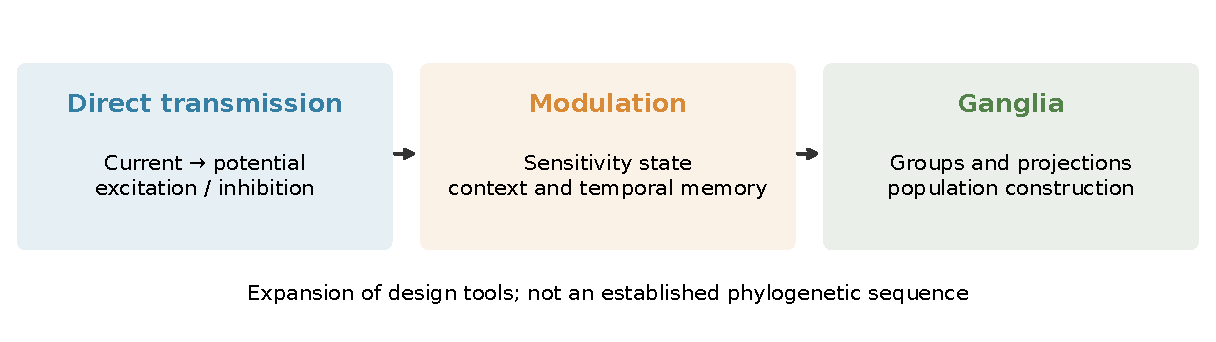
\includegraphics[width=\linewidth]{concept-en.pdf}
\caption{The proposed progression concerns available design tools. Modulation adds a dynamical sensitivity state; ganglia provide population organization and projection shorthand. The arrows do not assert a historical sequence in animal evolution.}\label{fig:concept}
\end{figure}

\section{Biological motivation and scope of the analogy}
The intuition ``direct transmission, then modulation, then ganglia'' is useful as a sequence of laboratory capabilities, but should not be treated as a universal biological ladder. Molecular components associated with synapses have antecedents predating neurons \citep{ryan2009}. The chemical-brain hypothesis explicitly considers diffuse chemical communication preceding synaptic wiring \citep{jekely2021}; work on early neural cell types likewise emphasizes secretory and transmitter-system diversification \citep{burkhardt2021}. Consequently, the appearance of modulation cannot be dated merely by placing it after direct synapses in a software interface.

Nervous-system centralization also has a branching and contested history. One account relates nerve cords and brains to the expansion and integration of earlier nervous centers \citep{arendt2016}. Comparative developmental evidence supports convergent origins of some bilaterian nerve cords \citep{martin2018}. These alternatives motivate studying organizing principles without claiming that a single sequence applies to all lineages.

We therefore use \emph{evolutionary capability} in a restricted sense: an available mechanism or representation may change the circuit configurations accessible to variation and selection. Demonstrating this change requires separating at least three propositions: a mechanism can express useful dynamics; a specific controller benefits from that mechanism; and a search process using it finds useful controllers more reliably. Our fixed-controller study tests the second proposition locally and characterizes the first at the implementation level. The third remains a hypothesis for future evolutionary experiments.

\section{Materials and methods}
\subsection{Laboratory architecture and experimental artifacts}
Spiking Bug consists of a Python simulation server and two TypeScript/Vite clients. The environment client displays the agent, food, pursuing threats, and physiological state. The connectome client supports neurons, synapses, ganglia, parameter inspection, and activity visualization. Both clients refer to one authoritative runtime. A portable JSON document contains topology, sensory and motor bindings, world parameters, and optional metadata. The editor permits explicit edges as well as ganglion projections that expand into individual edges before simulation.

The experiment uses source revision \code{befd6a0d53204722ade40be96000c3898b2158e5}. The three inputs are copied without parameter tuning from \code{direct.json}, \code{modulation.json}, and \code{ganglia-populatio.json}; the last filename is retained verbatim for reproducibility. The copies and their SHA-256 hashes are supplied with the data. All three have identical world descriptions and bindings. D has 11 sensory neurons, four motor neurons, and two additional neurons; M has four additional neurons; G contains 12 populations of 64 neurons and the same 15 sensory/motor neurons. All neurons in these inputs have zero intrinsic noise.

According to the author, the files were constructed by an agent identified as GPT-6 Astra. A common prompt requested survival for 20 minutes, starting with only the default sensory and motor neurons. The agent could create a saved circuit, test it, assess weaknesses, and iterate until an acceptable result. It could not change source code or environment settings, and neuron and synapse counts were unlimited. The permitted mechanisms differed between conditions: direct excitation/inhibition, additional modulation, and additional ganglion construction. The exact direct-only prompt was supplied by the author; the common base and differences in the other conditions are author-reported, not independently recovered generation logs. This is LLM-guided iterative optimization, not a single-shot generation or a biological evolutionary process. The shared prompt reduces variation in the stated task, but does not establish unbiased sampling, independent evolutionary replicates, or equal optimization effort. Model snapshot, sampling parameters, numbers of calls, tested candidates, selection history, and optimization seeds were not supplied. In particular, M changes direct wiring and neuron parameters as well as adding modulation. G changes size, parameters, and wiring. These differences are part of the artifact comparison and are not controlled away by using common environmental seeds.

\begin{table}[tbp]\centering\small
\caption{Structural inventory after projection expansion. Direct-edge signs refer to effective weights. ``Records'' count stored synapse objects, which need not equal individual edges.}\label{tab:structure}
\begin{tabular}{lrrr}\toprule
Property & D & M & G\\\midrule
Neurons &17&19&783\\
Ganglia &0&0&12\\
Stored synapse records &28&41&1887\\
Effective edges &28&41&3840\\
Positive direct edges &14&16&1856\\
Negative direct edges &14&23&1152\\
Excitation-modulating edges &0&2&640\\
Inhibition-modulating edges &0&0&192\\\bottomrule
\end{tabular}
\end{table}

\begin{figure}[tbp]\centering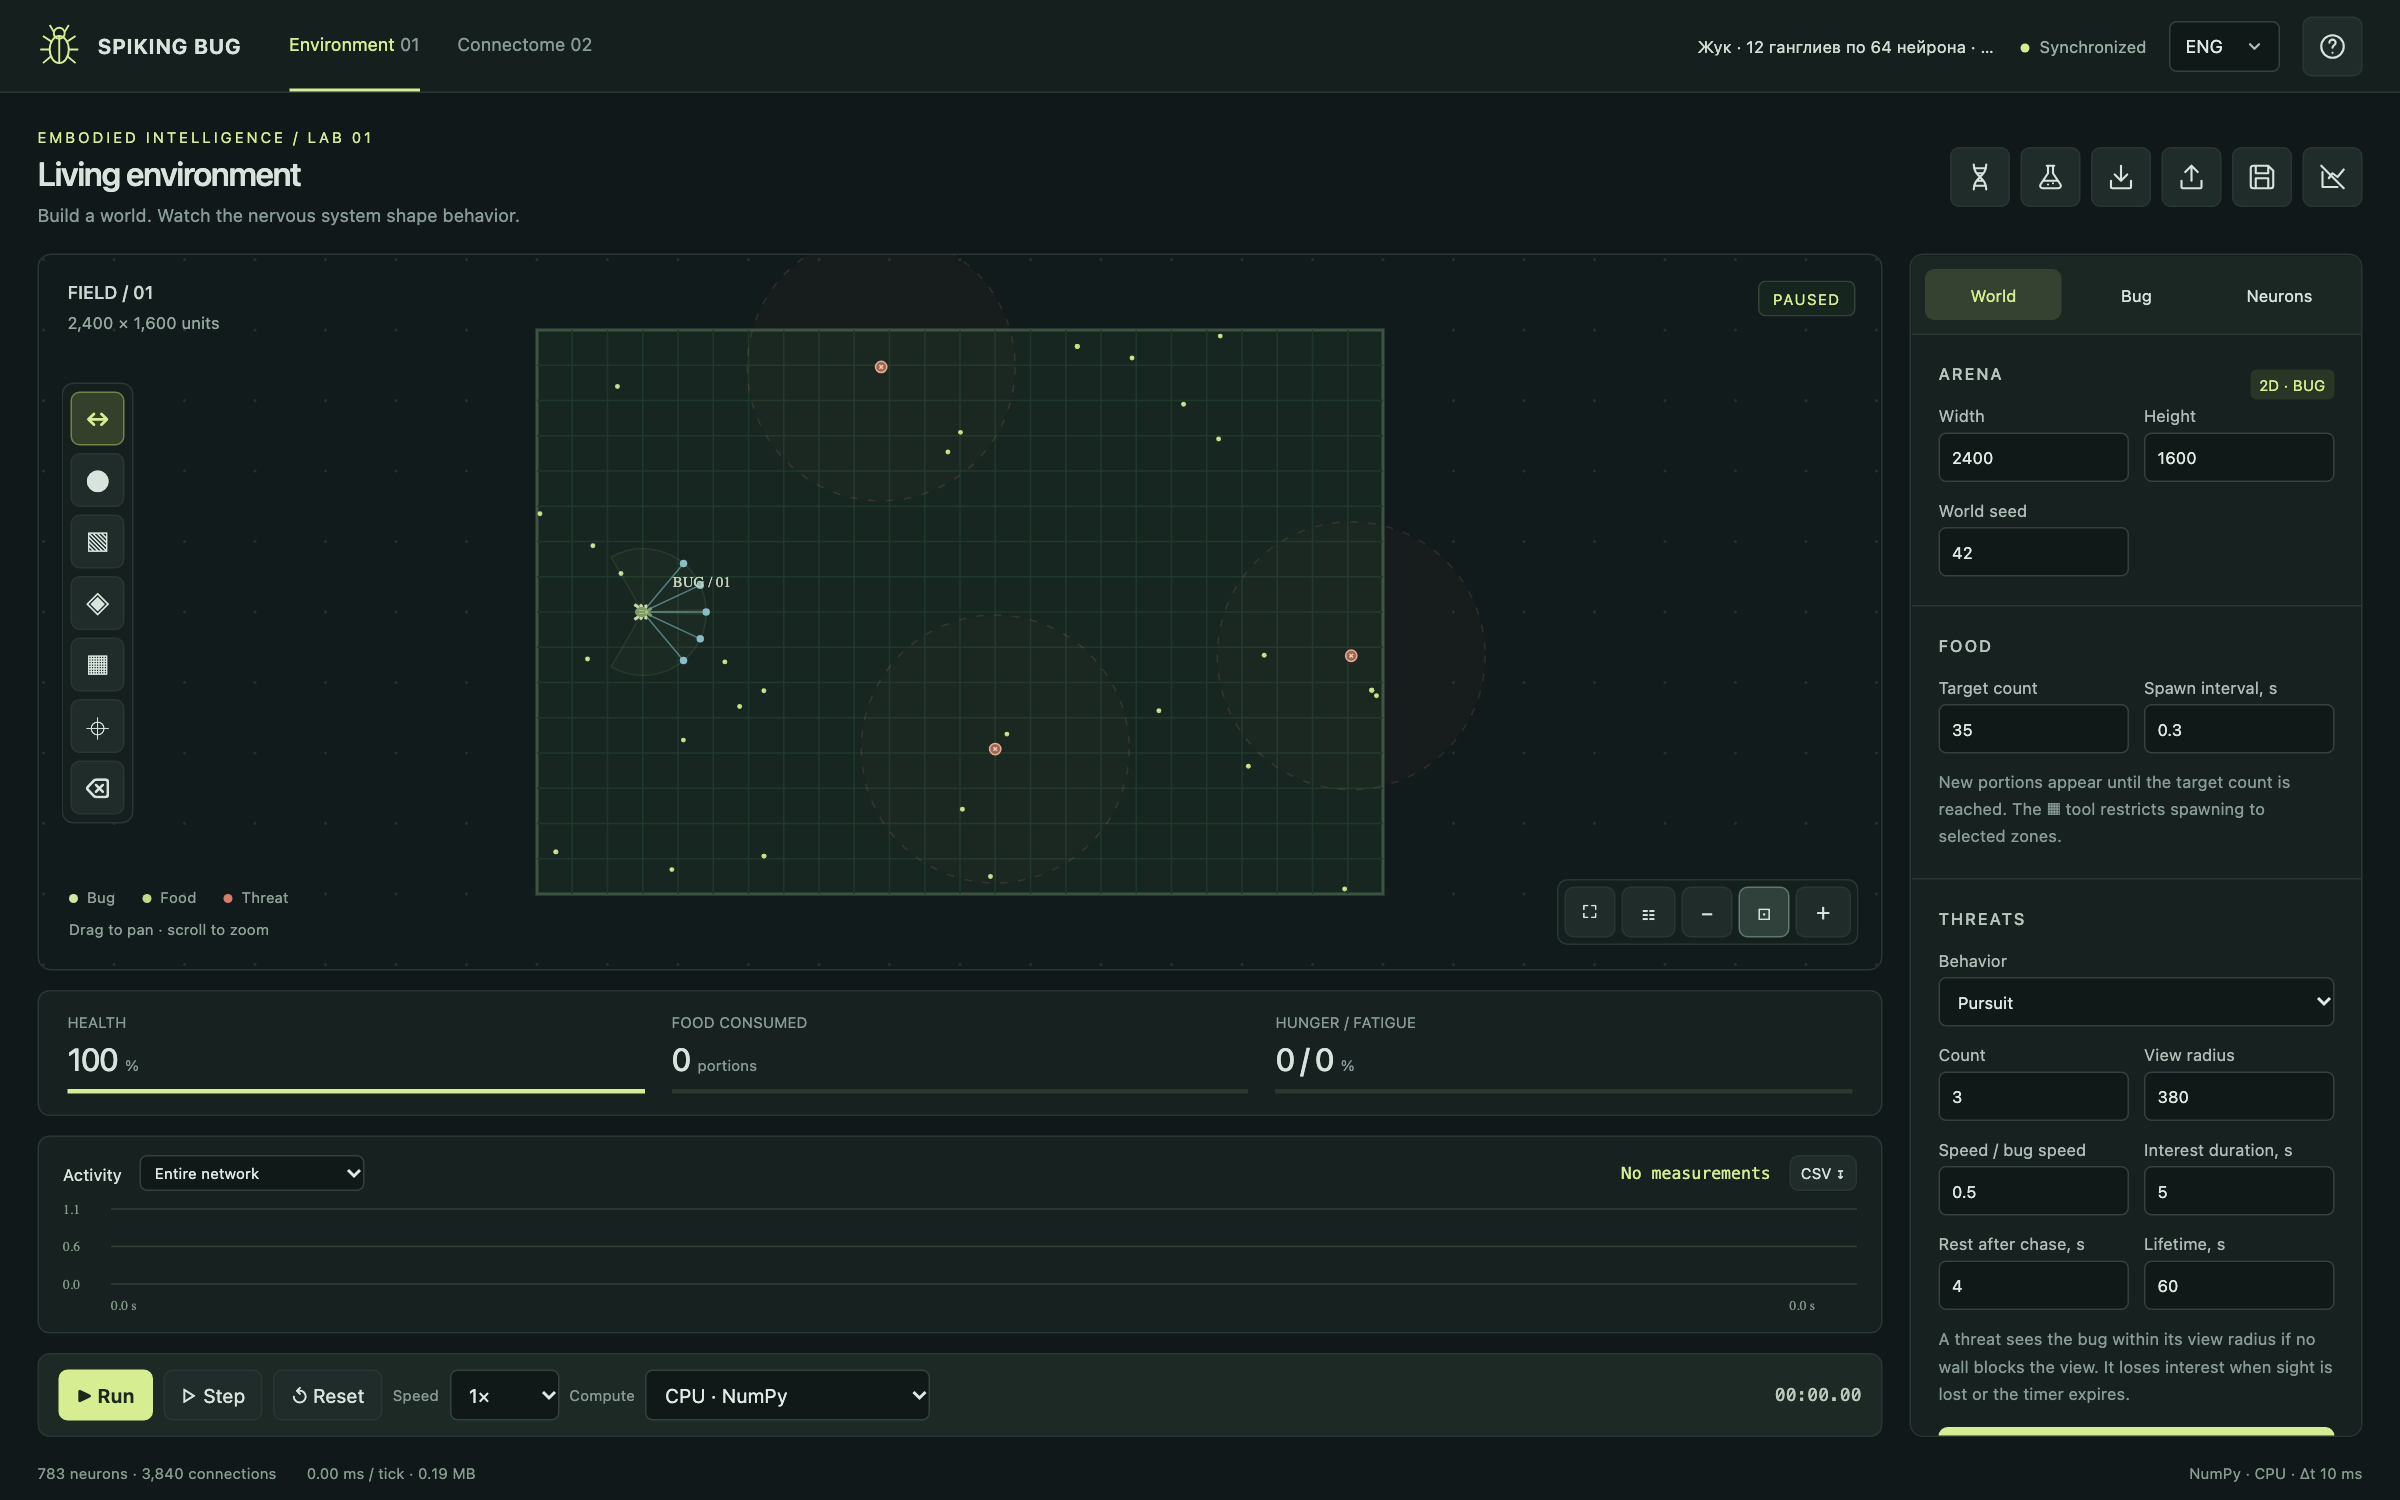
\includegraphics[width=\linewidth]{environment-en.png}
\caption{Actual environment interface, captured from an isolated local instance with controller G loaded. The saved scene is paused at $t=0$, seed 42. It illustrates the arena and tools; it is not a selected successful trial from the randomized evaluation. User-authored project labels retain their original language.}\label{fig:environment}
\end{figure}

\subsection{Discrete spiking dynamics}
The CPU/NumPy backend uses a fixed integration step $\Delta t=0.01$ s. Let $V_i^t$ denote membrane potential, $\lambda_i$ the per-step leak, $b_i$ bias, and $u_i^t$ sensory input. Delayed direct inputs are separated into positive and negative sums, $I_{i,+}^t$ and $I_{i,-}^t$, the latter being nonpositive. Two sensitivity variables $s_{i,+}$ and $s_{i,-}$ follow
\begin{equation}
\widetilde{s}_{i,q}^{t}=\operatorname{clip}_{[0,10]}\!\left[1+(s_{i,q}^{t-1}-1)e^{-\Delta t/\tau_{i,q}}+g_{i,q}M_{i,q}^{t}\right],\quad q\in\{+,-\},
\label{eq:mod}
\end{equation}
where $M_{i,q}^t$ is the sum of arriving modulatory weights and $g_{i,q}$ is a gain. The potential before thresholding is
\begin{equation}
\widetilde V_i^{t+1}=\operatorname{clip}_{[V_{i,\min},10^6]}\left[(1-\lambda_i)V_i^t+
\widetilde s_{i,+}^{t}I_{i,+}^t+\widetilde s_{i,-}^{t}I_{i,-}^t+b_i+u_i^t+\epsilon_i^t\right].
\label{eq:lif}
\end{equation}
The optional $\epsilon_i^t$ is zero in all evaluated inputs. A spike is emitted when the potential reaches threshold and the neuron was not refractory at the start of the tick. Refractoriness prevents emission but does not stop potential integration. In reset mode the implementation sets the potential to zero after emission; in retain mode it leaves the integrated value unchanged. The stored \code{v_reset} field does not supply a different reset value in this CPU path. The leak is a discrete coefficient, not a conductance measured in physical units.

A spike schedules its outgoing weights in a ring buffer with integer-tick delays. Modulation changes sensitivity to direct synaptic input, not sensory input or bias, and leaves the stored weights fixed. Thus this implementation is distinct from neuromodulated synaptic plasticity studied in evolutionary learning systems \citep{soltoggio2008}. Its internal state can carry recent context even without weight learning, but usefulness depends on the controller and task.

\subsection{Ganglia as a representation}
A ganglion is a named set of concrete neurons and an editor-level connector. A projection from a group of size $n_a$ to a group of size $n_b$ expands into $n_an_b$ individual edges. Each source member broadcasts its own spikes; there is no average ganglion signal, extra ganglion state, or additional group delay. For a direct projection from a ganglion, the sign of the weight may be assigned from the source neuron's excitatory or inhibitory polarity. This is why the effective graph must be counted after expansion.

If $\Phi$ is the expansion operator, the dynamics of a ganglion document $G$ are those of $\Phi(G)$. Grouping alone is therefore not a new neuron-level computation. It changes how a circuit is specified and manipulated. For unrestricted parameter budgets, adding optional modulatory edges contains direct-only networks as the zero-modulation case, $\mathcal H_D\subseteq\mathcal H_M$. By contrast, ganglion notation does not demonstrate a strict extension beyond the class of explicit graphs with the same mechanisms and neuron budget. Its potential advantage concerns representation, reuse, and the search induced by that representation.

\begin{figure}[tbp]\centering
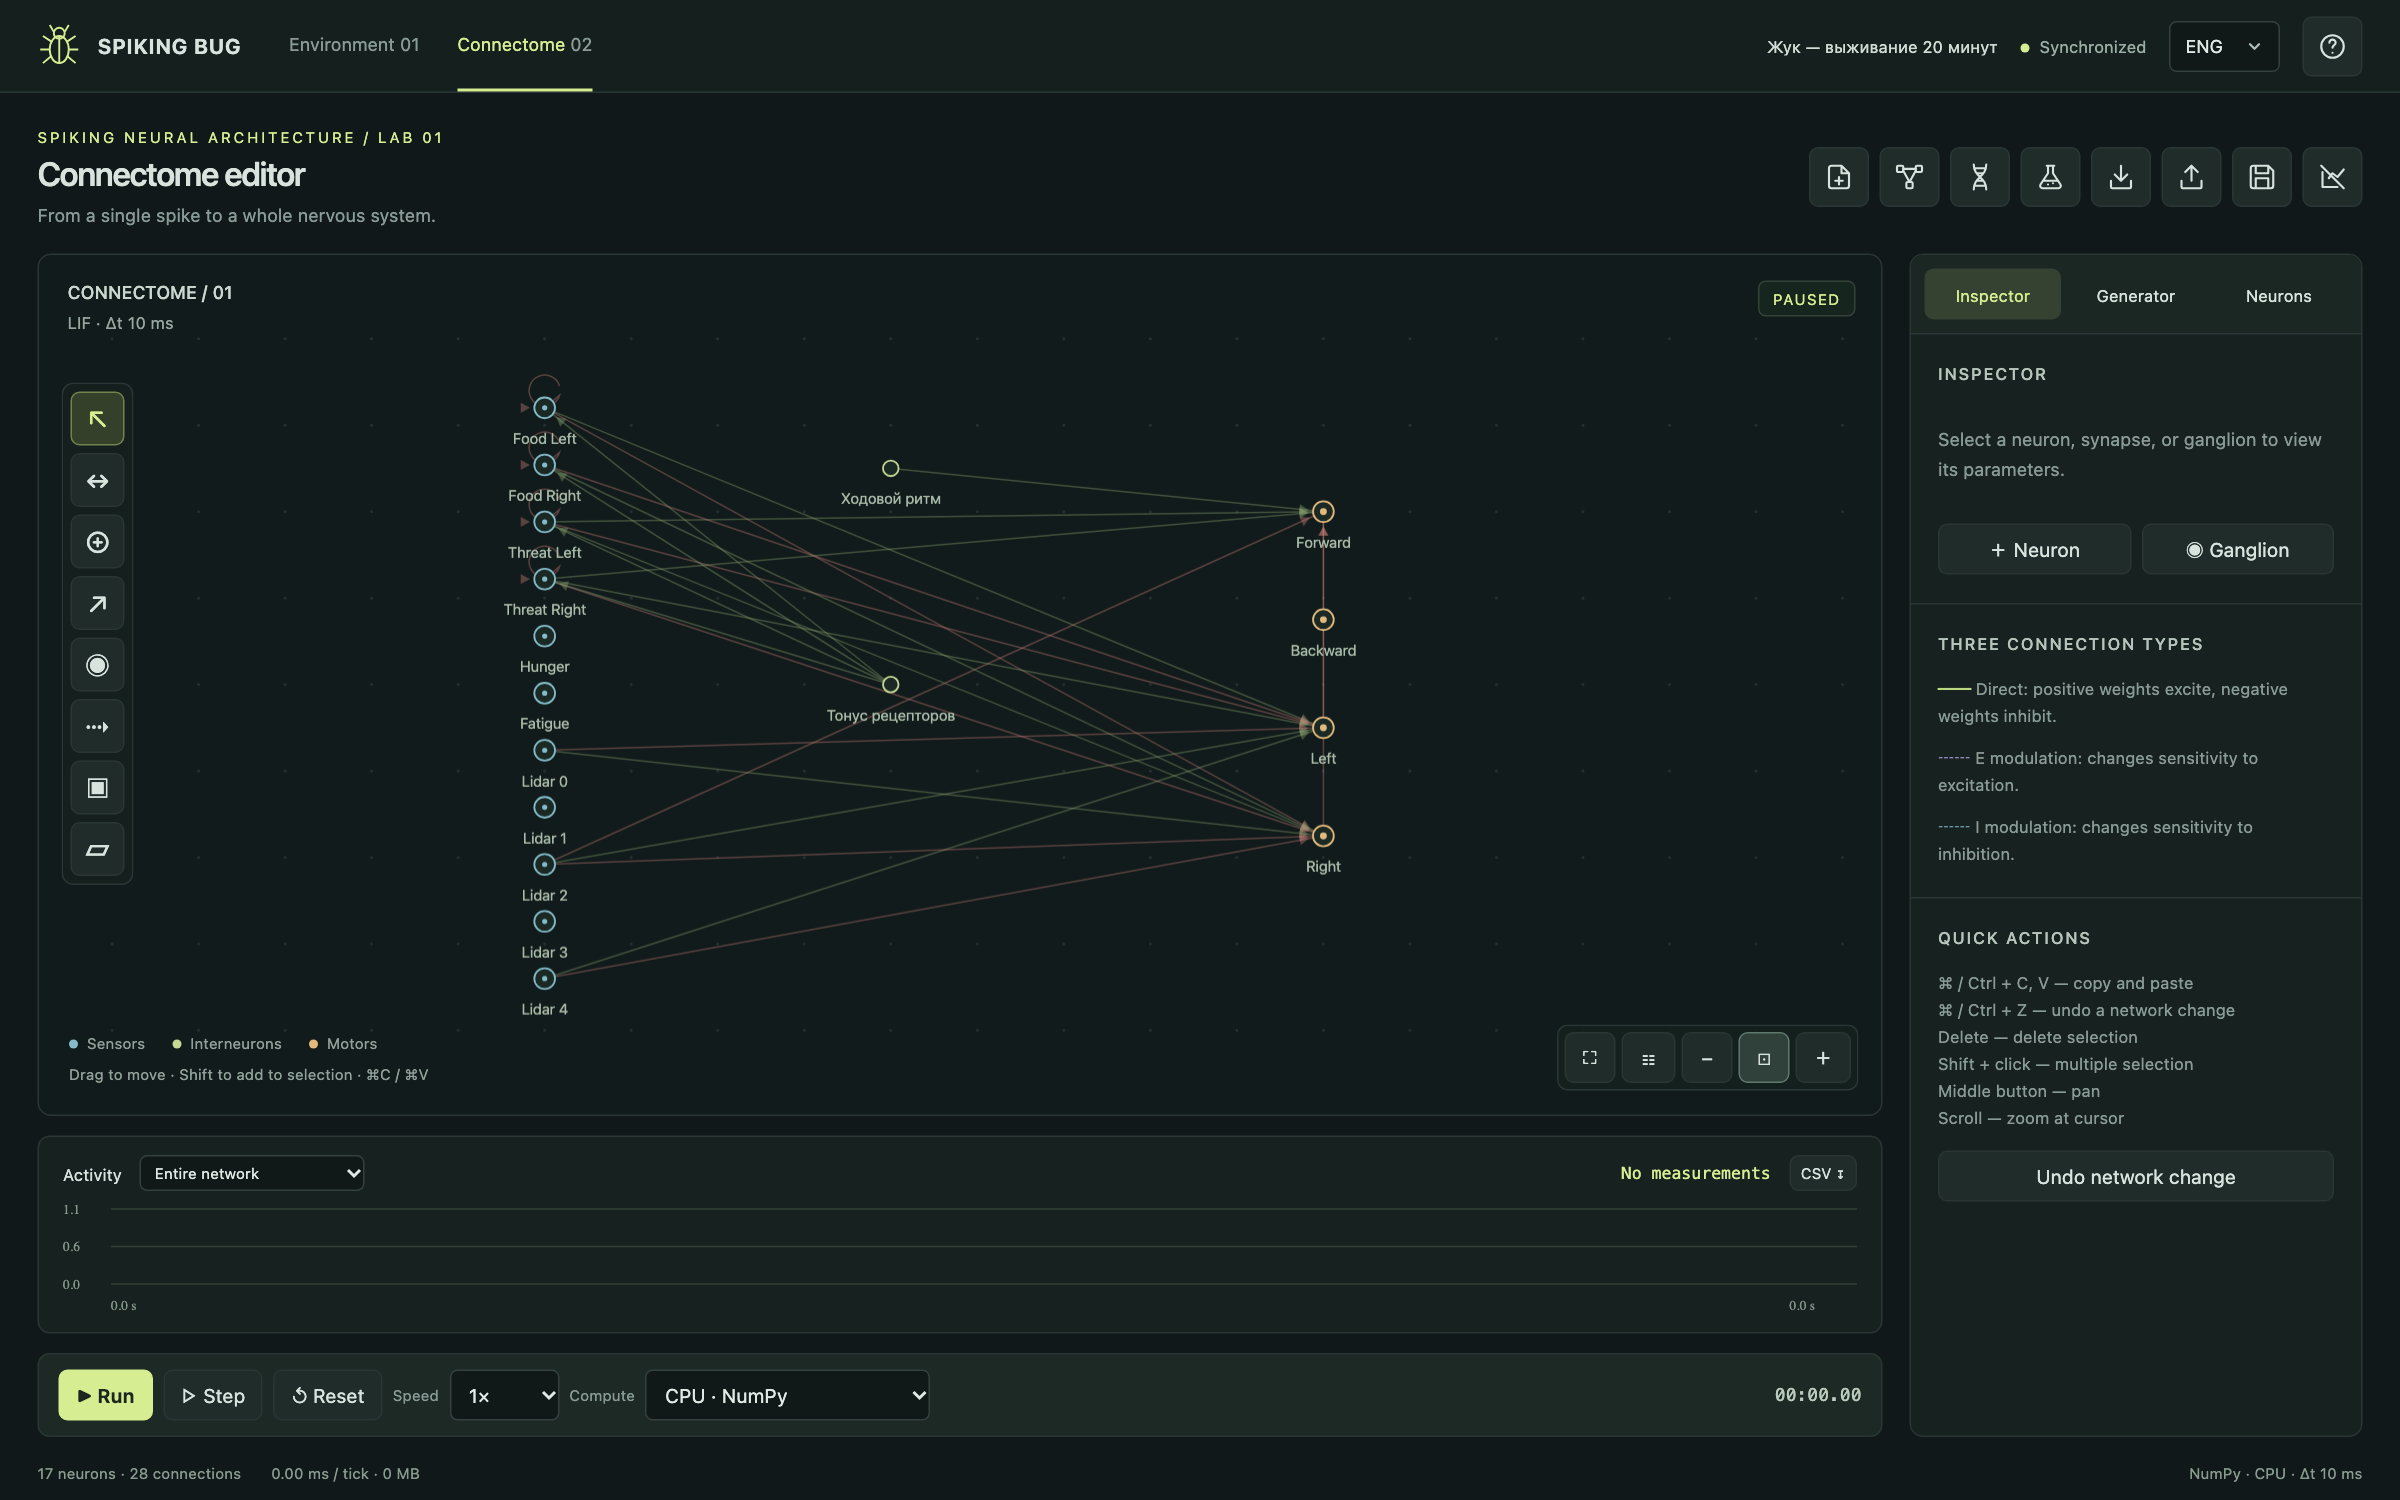
\includegraphics[width=0.98\linewidth]{editor-direct-en.png}\par\vspace{4mm}
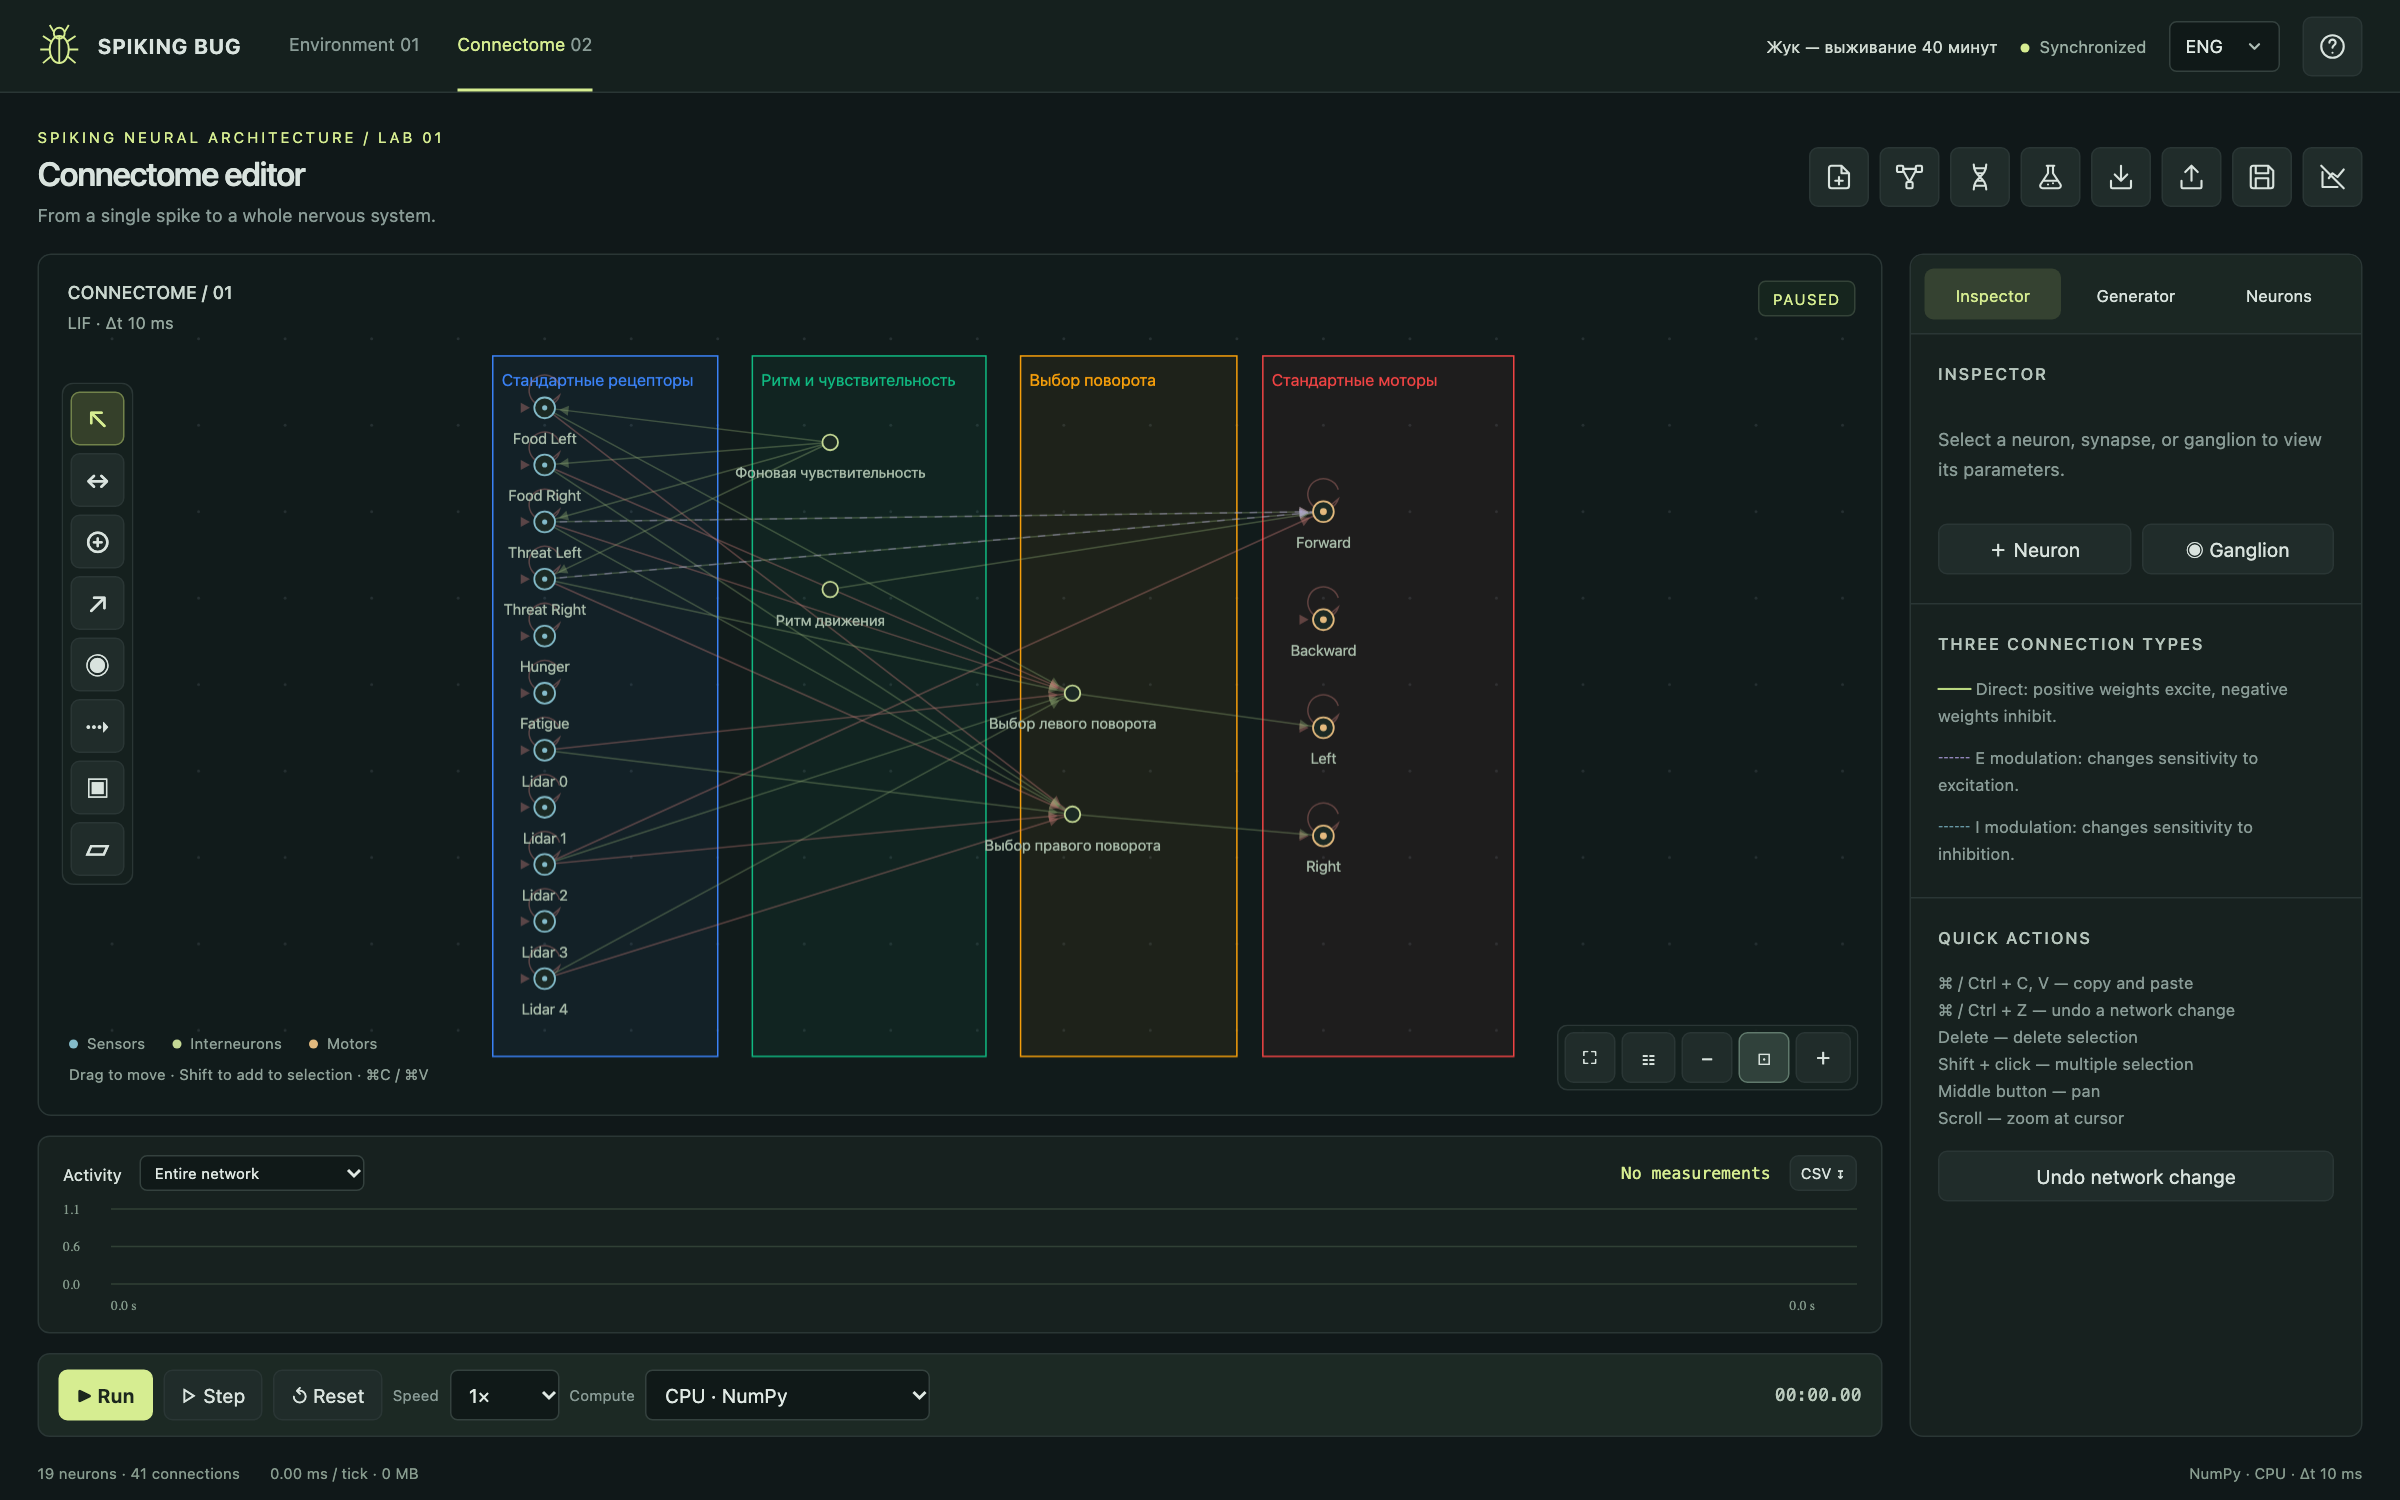
\includegraphics[width=0.98\linewidth]{editor-modulation-en.png}
\caption{The actual connectome editor with D (top) and M (bottom), each paused immediately after import. These are different complete designs, not an experiment in which only two modulatory edges were added to an otherwise fixed D network.}\label{fig:small}
\end{figure}
\begin{figure}[tbp]\centering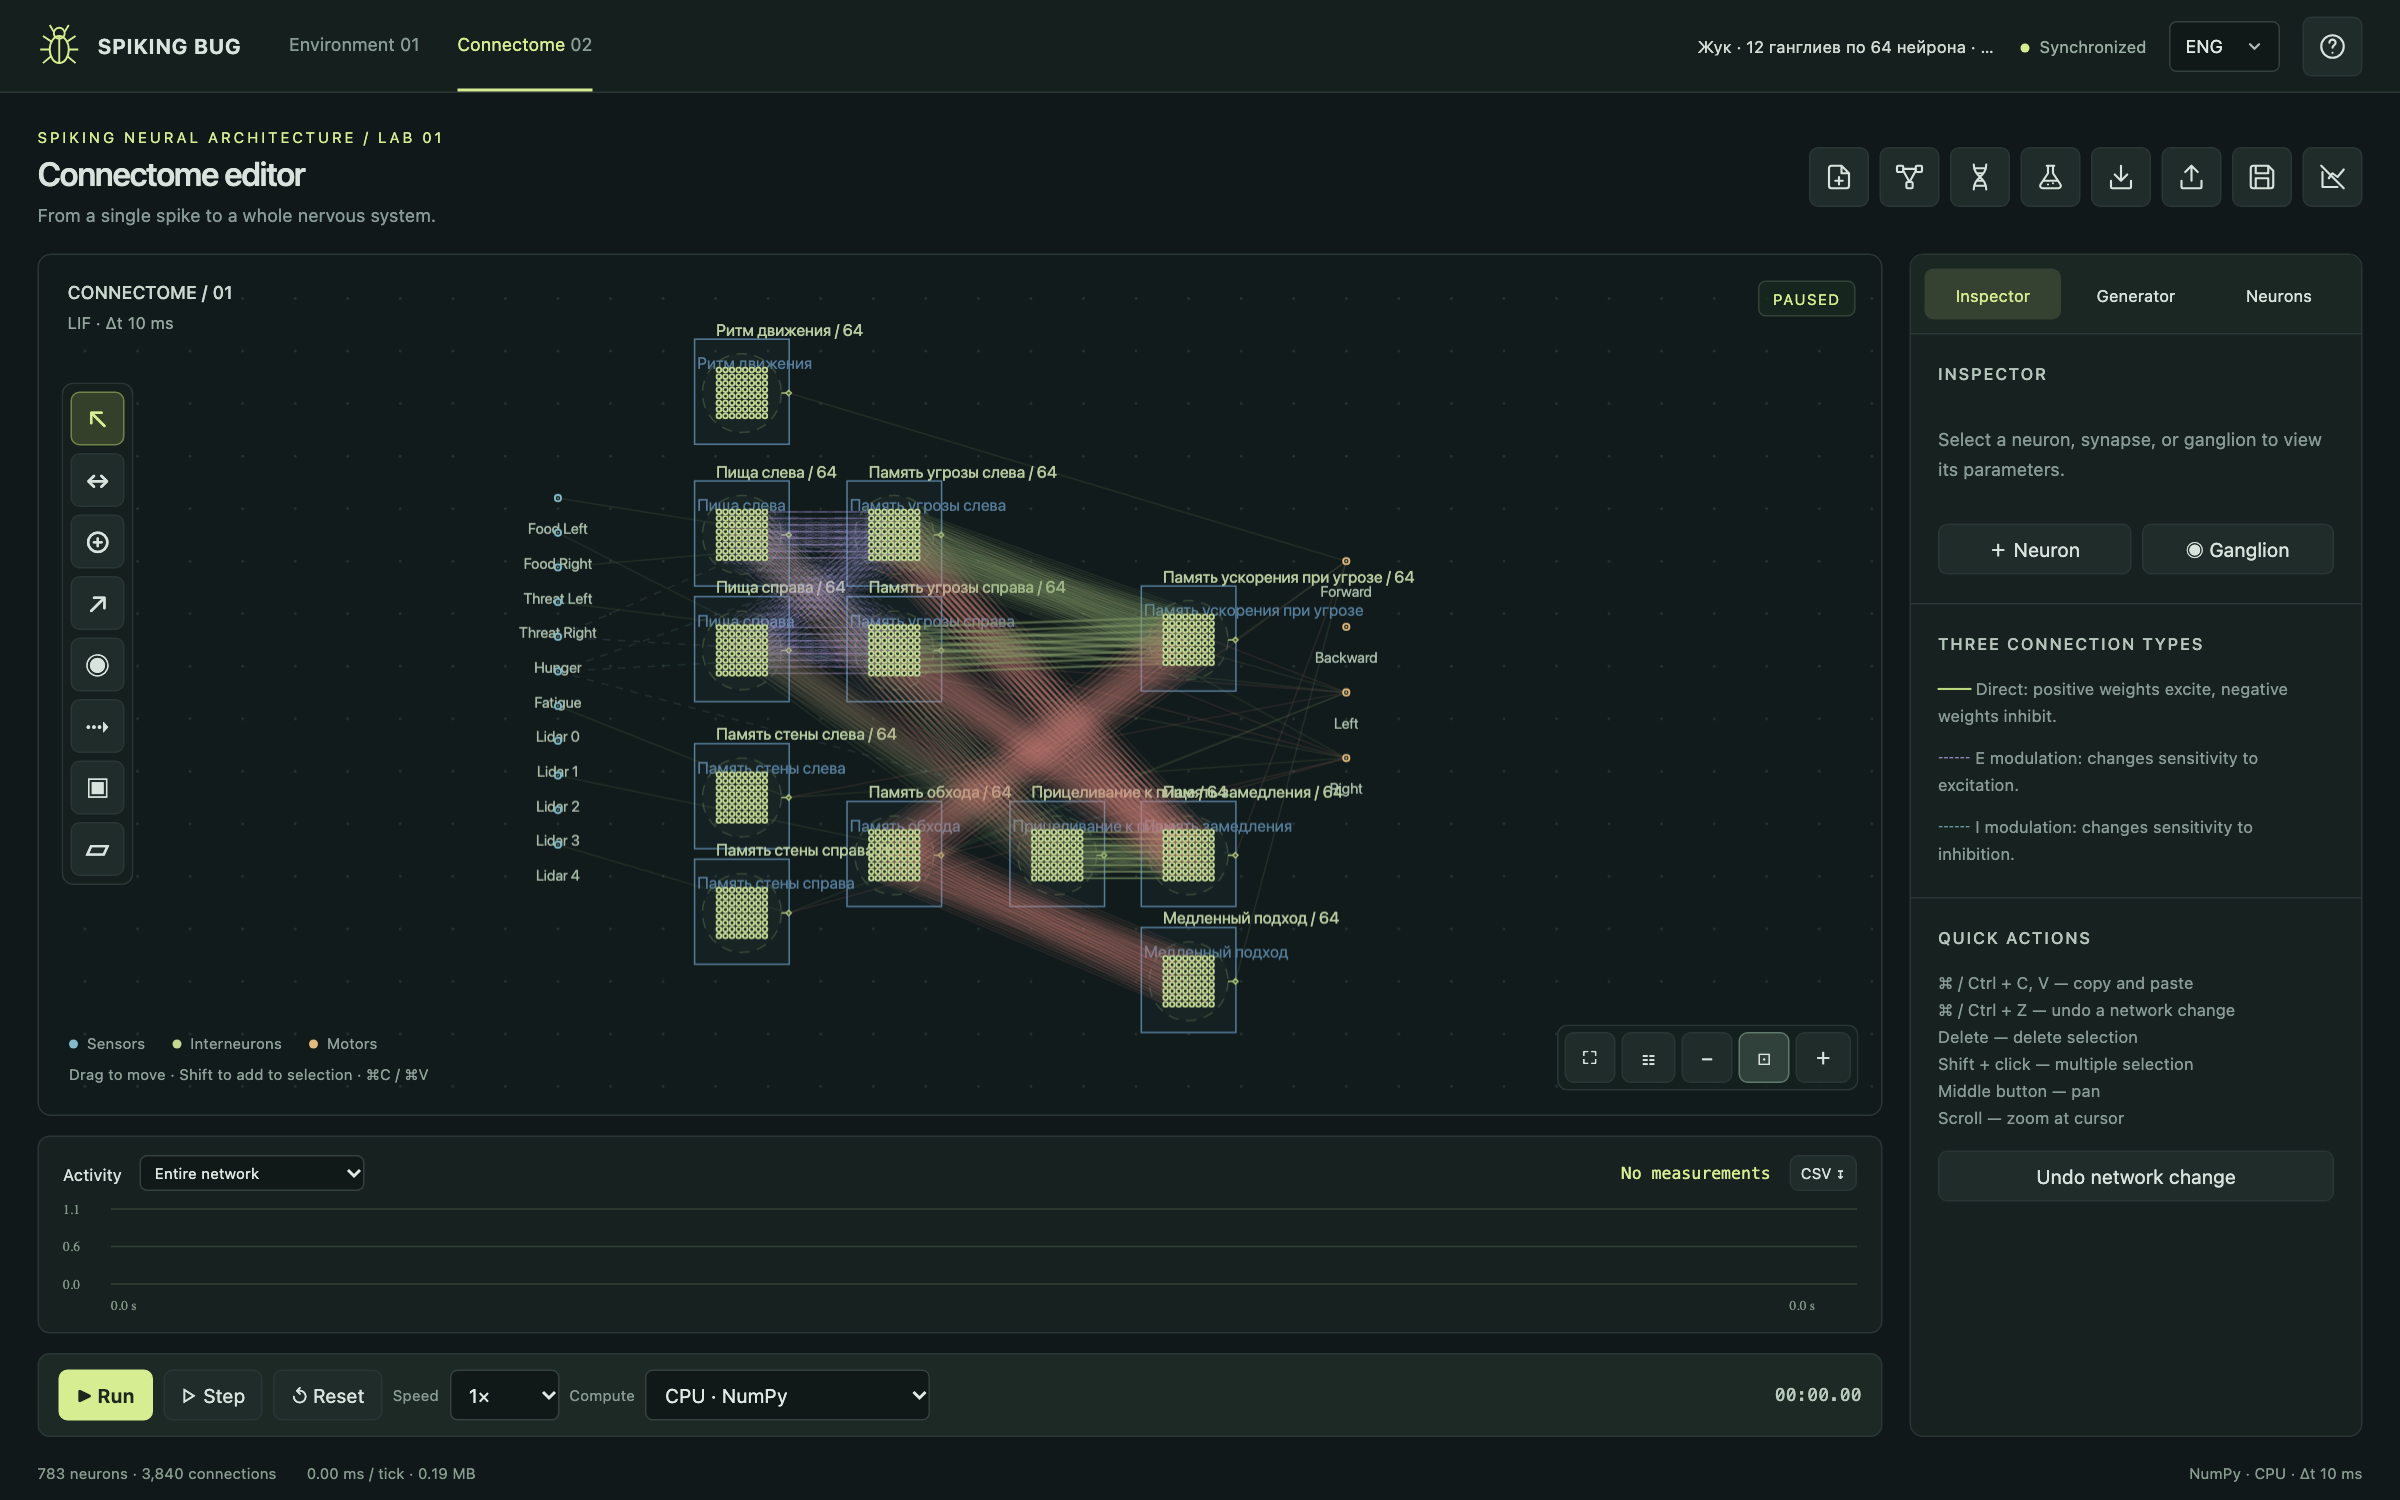
\includegraphics[width=\linewidth]{editor-ganglia-populatio-en.png}
\caption{The ganglion-based artifact G in the editor: 12 groups of 64 neurons, sensory and motor boundary neurons, and interpopulation projections. Original labels describe intended functions; they do not independently establish functional specialization. Dense labels are preserved as captured from the existing editor.}\label{fig:ganglia}
\end{figure}

\subsection{Embodiment and environment}
The arena is a bounded $2400\times1600$ space with a circular agent of radius 12. Eleven channels encode left/right food, left/right threats, hunger, fatigue, and five lidar directions. Four motor channels request forward motion, backward motion, and left/right turning. Binding depends on neuron identifiers, not labels or visual categories. Sensors are bounded in $[0,1]$ and their values are added to bound neurons each tick. Simultaneous commands are permitted.

Motor spikes are converted into discrete motion with a 0.04-s command duration within a 0.01-s world tick. With the configured speed of 150, a forward event requests six spatial units; backward motion has a factor of 0.7. A turn event requests $3\times0.04=0.12$ rad. Thus nominal speed alone does not describe the agent's effective speed: spike timing, refractoriness, simultaneous commands, and collisions matter. Pursuers move with the world step and a nominal speed ratio of 0.5.

Food contact resets hunger and restores up to 0.12 health. Hunger grows by 0.02 per second; at full hunger health decreases by 0.015 per second. Threat contact removes 0.25 health per second. Threats have a visibility radius of 380, a five-second pursuit interval, four-second rest, and 60-second lifetime. The target population is 35 food items and three threats; food replenishment is checked every 0.3 s. There are no internal obstacles or food zones in the three supplied worlds, so this study does not evaluate the available maze editor.

Fatigue is updated as
\begin{equation}
 f_{t+1}=\operatorname{clip}_{[0,1]}\left[f_t+\gamma\sum_k a_k^t+\rho N\Delta t-\delta\Delta t\right],
\end{equation}
with motor indicators $a_k^t$, $\gamma=0.025$, recovery $\delta=0.07\,\mathrm{s}^{-1}$, neuron count $N$, and neural-cost coefficient $\rho$. The motor term is per command event, not multiplied by $\Delta t$. Actual translation or rotation at full fatigue costs 0.01 health per second. At $\rho=0$ the default environment does not charge for neuron count. These numerical costs are simulator rules, not a calibrated metabolic model.

\subsection{Protocol, controls, and endpoints}
The primary comparison evaluates D, M, and G on seeds 21000--21059 with a horizon $\tau=1200$ s. An initial 600-s evaluation used the same seed panel and was completed and inspected. After the author supplied the original 20-minute design target, the evaluation was extended to 1200 s without modifying the controllers or choosing a new seed panel. The earlier results are retained separately. This is a transparently amended descriptive evaluation, not a preregistered or untouched confirmatory test. A single timing pilot at seed 9000 and 120 s was excluded. Controllers were not tuned during this evaluation. Because the original optimization seeds are unavailable, overlap with the agent's earlier tests cannot be ruled out; the panel is not claimed to be verified held-out from design. Initial food and threats are regenerated by the native trial routine while retaining obstacles, spawn pose, and configuration. The same seed gives each controller the same initial placement. Later random draws can diverge when behavior changes food replenishment or threat replacement, so this is seed pairing rather than a claim of identical complete external trajectories.

Each episode constructs a fresh network and world, runs without wall-clock pacing, and terminates at the first zero-health state or at the horizon. This differs from the interactive environment, where motion may continue after zero health and later food may restore it. We use the native first-death evaluation semantics. Sixty seed blocks are the replication units; time steps are not independent replicates.

Two secondary interventions remove every \code{mod_exc} and \code{mod_inh} edge from M or G, keeping neurons, direct edges, and their parameters unchanged. Three further conditions repeat D, M, and G at $\rho=0.001$ per neuron per second. This produces $8\times60=480$ episodes. The cost condition is a single sensitivity analysis, not a calibrated energy comparison. Three additional G replays compare the grouped document with its expanded explicit graph on seeds 21000--21002. A fixed-seed diagnostic compares the intact and ablated M spike sequences under the intact closed-loop input stream. Three separate descriptive trials use the original saved scene, seed 42, without initial randomization.

The primary survival endpoint is restricted mean survival time (RMST),
\begin{equation}
\widehat{\operatorname{RMST}}(\tau)=\frac{1}{n}\sum_{j=1}^n\min(T_j,\tau),
\end{equation}
which here equals mean recorded duration because censoring occurs only at the common horizon. Its interpretation does not require extrapolating unobserved lifetimes \citep{royston2013}. We also report survival to 1200 s, food count accumulated until termination, food per minute alive, distance, terminal health, collision blocking, and mean firing frequency. The runtime's damage counter includes threat and exhaustion damage but excludes starvation loss; it is therefore not total health loss. Food per minute is conditional on time alive and must be read together with survival.

For continuous endpoints we use 20,000 seed-block bootstrap resamples and percentile 95\% confidence intervals (random generator seed 20261021). Pairwise contrasts resample paired differences. Survival proportions receive Wilson 95\% intervals. Intervals describe variation across scenes for these fixed controllers, not uncertainty over independently designed networks. All secondary contrasts are exploratory, intervals are pointwise, and no multiplicity-adjusted significance claim is made. No episode is excluded on the basis of its outcome. Computation uses CPU/NumPy; the exact software versions and host metadata are recorded in the protocol file.

\section{Results}
\subsection{Behavioral ordering of the original designs}
Table~\ref{tab:baseline} and Fig.~\ref{fig:performance} show a pronounced ordering in food collection: D averages \DFood{}, M \MFood{}, and G \GFood{} portions per episode. The paired M--D difference is \MDdiff{} portions (95\% CI \MDlo{} to \MDhi{}), and the G--M difference is \GMdiff{} (\GMlo{} to \GMhi{}). These are comparisons of the complete designs under one shared environment family.

A separate descriptive control on the original saved scene at seed 42 yields survival to 1200 s for all three controllers and food counts of 67, 212, and 399. These three episodes are not pooled with the randomized panel. Meeting the original objective in one saved scene is therefore compatible with weaker robustness across randomized scenes.

Survival improves substantially between D and the two richer designs, but is not strictly ordered by design complexity. D survives to the horizon in \DSurv{}/60 episodes, while M and G do so in \MSurv{}/60 and \GSurv{}/60. Their RMST values are \DTime{}, \MTime{}, and \GTime{} s. All M episodes and all but one G episode reach the horizon, producing a substantial survival ceiling. G has one more observed death than M; this does not support a monotonic survival advantage with increasing complexity. The restricted means do not establish unrestricted lifetimes or robustness in harder environments. In particular, greater food collection cannot be relabeled as demonstrated superiority in lifespan.

\input{data/baseline-en}
\begin{figure}[tbp]\centering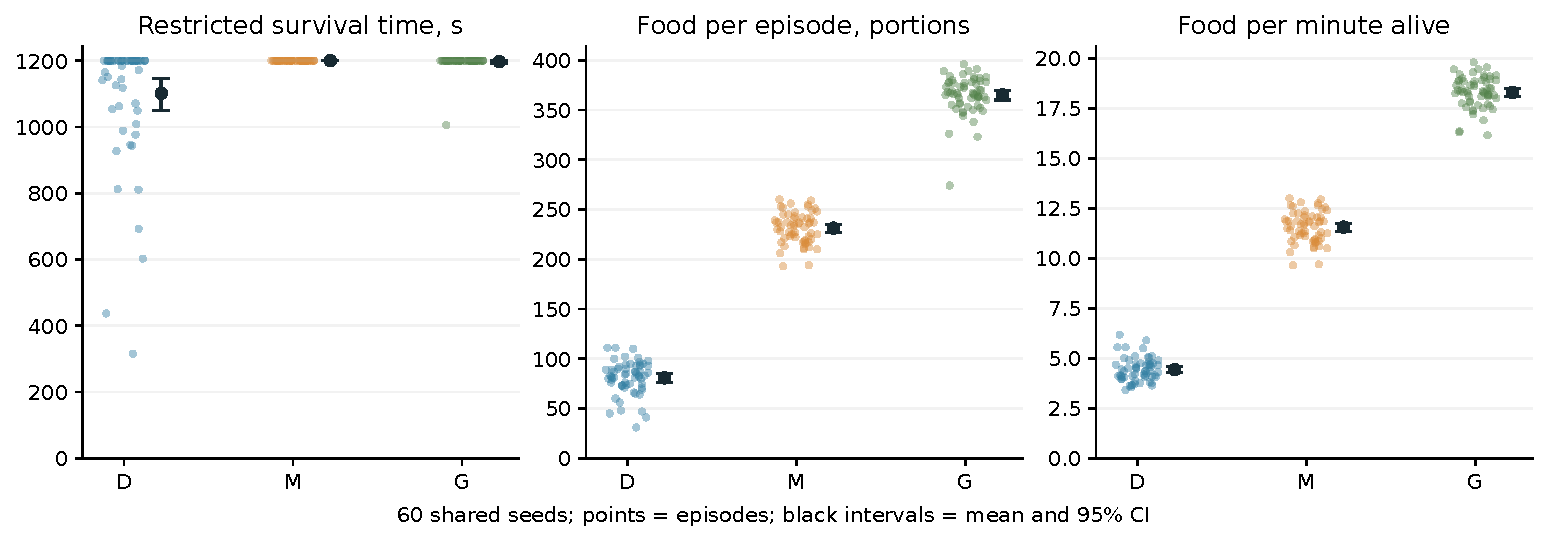
\includegraphics[width=\linewidth]{performance-en.pdf}
\caption{Original-controller performance on 60 paired seeds. Colored dots are individual episodes; black points and intervals show means and bootstrap 95\% intervals. Survival duration is capped at 1200 s. Food rate uses time alive as its denominator.}\label{fig:performance}
\end{figure}

\subsection{Modulation ablations}
Removing M's two excitation-modulating edges produces exactly the same recorded duration, food count, food rate, health, damage, distance, blocking, and firing frequency on every seed. This is stronger than failure to detect a difference in a sample mean, but it remains limited to this input panel and these measured outcomes. The seed-21000 trace diagnostic confirms \TraceMismatch{} ticks with differing spike vectors out of 120,000, even though forward-neuron sensitivity changes on \TraceModTicks{} ticks and reaches \TraceMaxSens{}. The forward neuron emits 29,999 spikes in 1200 s (24.999 Hz), essentially its 25-Hz ceiling imposed by three refractory ticks plus the emission tick. This supports a saturation explanation for this diagnostic: additional positive drive need not increase an already maximal spike rate. Thus a functioning modulatory state can be behaviorally redundant under the tested conditions.

In G, removing all modulation increases mean food collection from \GFood{} to \GNoModFood{} portions, while survival increases from 59/60 to 60/60. The paired intact-minus-ablated difference is \GAblDiff{} portions (95\% CI \GAblLo{} to \GAblHi{}). For this design and task family, modulatory connections therefore do not explain the advantage over M; their net contribution to food collection is adverse. This does not show that modulation is generally harmful. It shows that availability of a mechanism and beneficial use of that mechanism are different claims. The intact network was not retuned after ablation, and the observed gain is not an estimate of the best achievable direct-only policy.

\input{data/controls-en}
\begin{figure}[tbp]\centering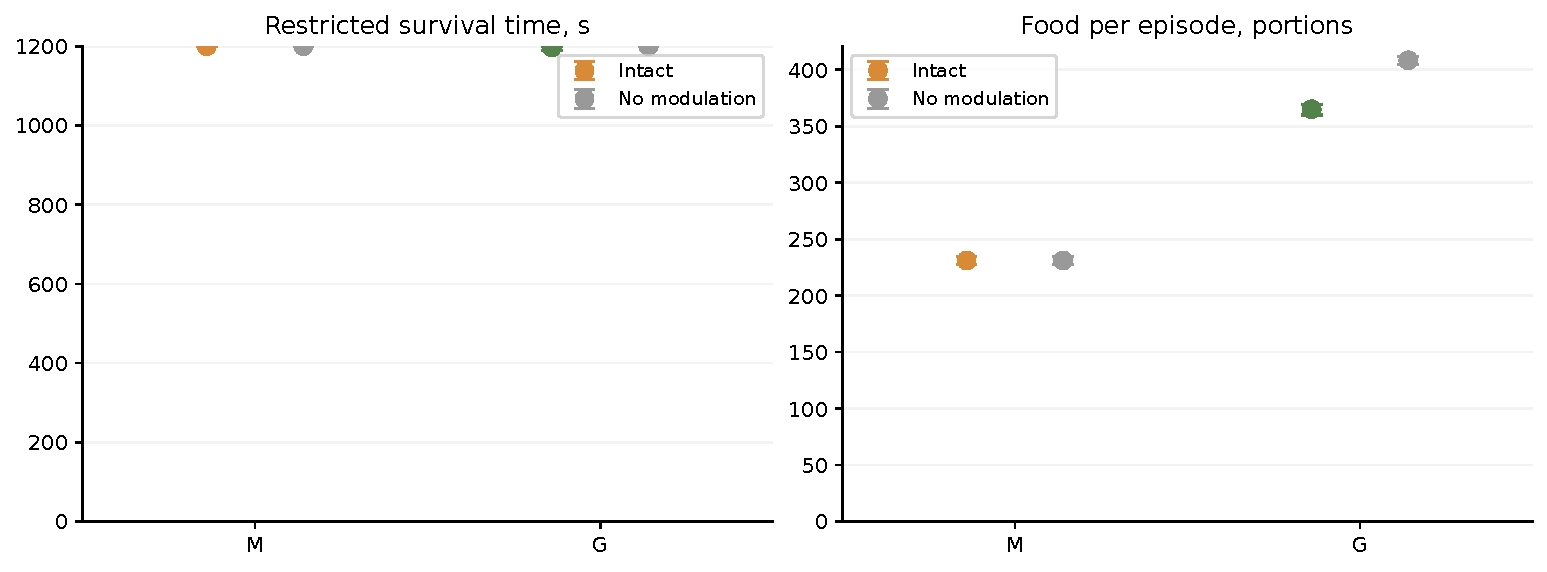
\includegraphics[width=\linewidth]{ablation-en.pdf}
\caption{Mechanism-removal controls. Points show the intact and modulation-ablated M and G means with 95\% bootstrap intervals. The interventions preserve neuron count and all direct synapses.}\label{fig:ablation}
\end{figure}

\subsection{Grouping, resources, and the cost condition}
The flattened G graph has 783 neurons and 3840 effective edges, with no ganglion objects. All recorded behavioral outcomes exactly match the original in the three designated replay checks. This is consistent with the expansion semantics: a ganglion is a constructional abstraction over concrete neurons, not an extra dynamical primitive. The replay check establishes implementation equivalence for the tested seeds; the equality of the intended graphs is the broader structural explanation.

G uses approximately 46.1 times as many neurons as D and 41.2 times as many as M. Its larger raw food count is therefore not a statement of better resource efficiency. Dividing each controller's mean food count by its number of neurons gives \DFoodPerNeuron{}, \MFoodPerNeuron{}, and \GFoodPerNeuron{} portions per neuron per episode for D, M, and G. This normalization is only a descriptive proxy; it does not measure energy or a biological optimum. Neural signaling has several distinct energetic costs \citep{attwell2001}, none of which are captured adequately by a bare neuron count.

At $\rho=0.001$, the imposed fatigue increments before recovery are 0.017, 0.019, and 0.783 per second. Table~\ref{tab:cost} reports the outcomes without conflating that penalty with energy. Duration, food collection, terminal health, and distance are identical to baseline seed by seed in all three controllers; cumulative damage and firing statistics do change in subsets of episodes. Thus the intervention is active, but does not discriminate the main behavioral endpoints in this panel. The bounded fatigue state and its dependence on movement can make a substantial change in nominal cost have a comparatively small behavioral effect; a null or small change here cannot establish that large networks are metabolically cheap.

\input{data/cost-en}
\begin{figure}[tbp]\centering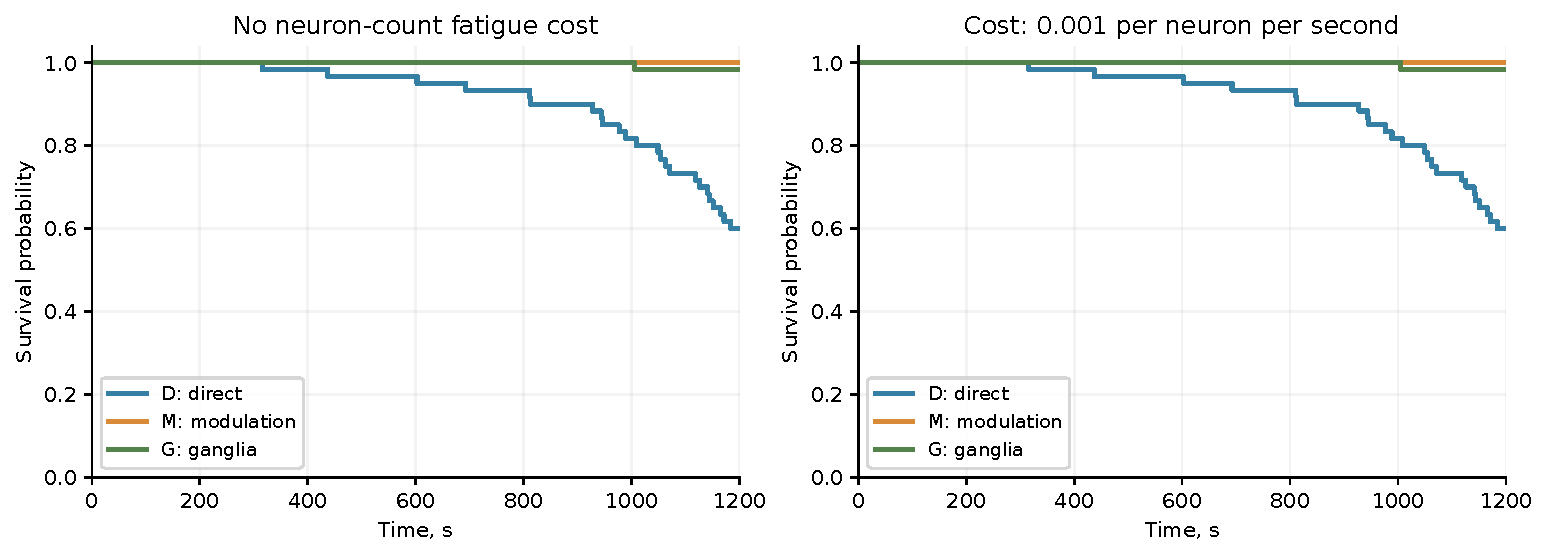
\includegraphics[width=\linewidth]{survival-en.pdf}
\caption{Empirical survival curves without neural-count cost and under the single cost condition. All censoring occurs at the common horizon. Curves at one indicate no deaths observed before 1200 s, not indefinitely sustainable behavior.}\label{fig:survival}
\end{figure}
\begin{figure}[tbp]\centering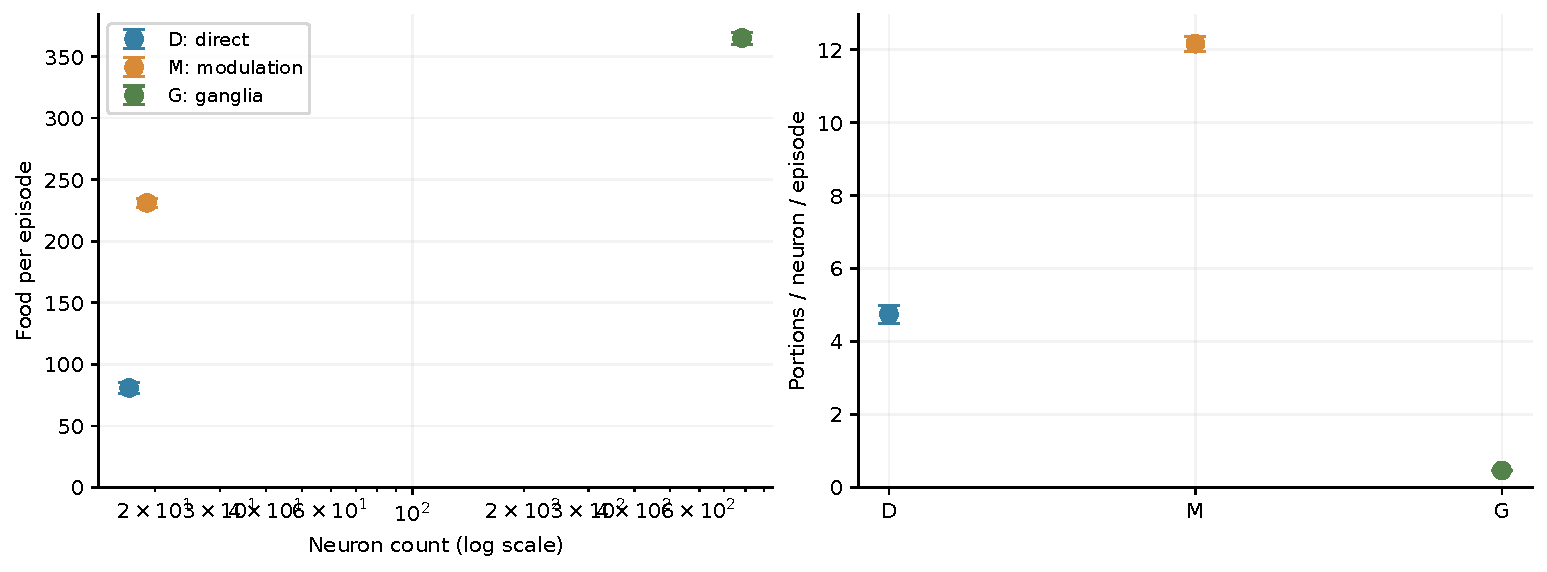
\includegraphics[width=\linewidth]{resources-en.pdf}
\caption{Raw collection performance versus neuron count (left) and food count divided by neuron count (right), with bootstrap 95\% intervals. The left panel uses a logarithmic neuron-count axis. The right panel is a resource-normalized descriptor, not an energy measurement.}\label{fig:resources}
\end{figure}

\section{Discussion}
\subsection{What the progression demonstrates}
The three artifacts illustrate a useful progression in the designer's available vocabulary. Direct interactions specify immediate positive and negative influences; modulation adds context-sensitive gain dynamics; populations provide a way to construct and connect repeated neural structures. This progression makes it possible to ask more structured questions about behavior and representation. It does not entail a monotonic increase in performance for every network or every metric.

The raw food-collection ordering is real in the evaluated panel of LLM-designed artifacts. Its cause is not identified by the original comparison, because network size, direct weights, leak, bias, and connectivity also vary. The ablations substantially narrow the interpretation: M's measured improvement over D survives complete removal of modulation, and G's food count improves when modulation is removed. It would therefore be incorrect to present the main bar or point plot as evidence that adding modulatory synapses caused the observed improvement.

This negative mechanistic result strengthens the study's methodological message. A model can implement a biologically motivated capability correctly without a supplied example exploiting it advantageously. A representation may make complex designs convenient without its grouping operation altering the expanded circuit's behavior. Evaluating intermediate mechanisms prevents an attractive evolutionary narrative from becoming an unsupported causal explanation.

\subsection{From capability to evolvability}
Evolutionary algorithms can modify architectures and parameters under a selection criterion \citep{floreano2008}. Spiking Bug also contains an optional mutation-and-selection subsystem, but no evolutionary search was conducted for the reported results. Generation curves, search efficiency, adaptation speed, and evolved novelty are consequently not claimed. Source-level availability of that subsystem does not convert this fixed-controller comparison into an evolutionary experiment.

A direct test of evolvability would require independently initialized searches in each representation, frozen training and validation scenarios, and a final untouched test panel. Population size, evaluation budget, neuron/edge budgets, and mutation opportunities should be matched or reported as separate factors. Multiple evolution seeds are needed; sixty environments for one controller cannot replace sixty independent lineages. Group-level mutation or duplication could then be tested against explicit-graph mutation, using the same expanded resource budgets. Under such a design, the hypothesis becomes measurable: do richer construction rules increase the probability or speed of reaching a specified held-out performance threshold?

For LLM-assisted construction, an analogous but separate design is needed: independent agent sessions per condition, a fixed system context, equal numbers of model calls and simulator trials, archived candidates, and a common stopping criterion. A shared prompt is useful but does not by itself ensure these controls. The current results concern the three resulting artifacts, not the distribution of GPT-6 Astra design success.

\subsection{Task dependence and biological interpretation}
The current open arena favors sustained resource acquisition with limited sensory channels. It does not test delayed reward, context reversal, multi-stage decisions, maze generalization, or transfer between ecologies. Such tasks may provide stronger reasons for a decaying modulatory state or reusable population structures. Their inclusion must be decided before selecting favorable results; post hoc task choice could otherwise create an apparent mechanism advantage.

Biologically, the appropriate analogy is an expansion and reorganization of possible control mechanisms under ecological constraints. The data do not establish a historical order of neurotransmitter appearance, ganglion evolution, or centralization. They also do not support a universal increase in complexity: a compact controller can be more economical on a given task. The literature on diffuse chemical signaling and convergent nervous-system organization is compatible with diverse trajectories, rather than a single march from simple to complex \citep{jekely2021,martin2018}.

\subsection{Limitations}
The principal limitation is one controller per design category. All statistical intervals condition on these exact artifacts. Shared prompting is a control on instructions, not a guarantee of impartiality: the LLM may introduce architectural preferences, and different design runs may use different amounts of simulator feedback. The experiment measures robustness to scene randomization, not a population-level effect of architectural class. The original numbers of LLM iterations, trial seeds, selection criteria, and resource usage are unknown. Unlimited circuit size is faithful to the supplied design prompt, but does not make the capacities equal. The large difference in network size confounds capability with capacity, and no matched-size direct-only network was optimized as a competing design.

The absence of internal obstacles limits claims about navigation. The finite horizon limits claims about survival. The single neural-cost coefficient does not identify a performance--energy frontier. Zero intrinsic neural noise restricts stochastic variability to the environment. CPU execution has been evaluated; GPU numerical agreement and hardware energy were not measured. Finally, the simplified neuron, scalar sensitivity, and planar body are functional abstractions; no biological species or anatomical connectome is reconstructed.

\section{Conclusion}
Spiking Bug provides a common executable setting for exploring direct transmission, modulatory sensitivity, and population-based circuit construction. Three supplied designs show a pronounced increase in food collection under a paired 60-scene evaluation. Survival distinguishes the simple controller from the two richer designs, with no monotonic M-to-G gain and substantial censoring at 1200 s. Mechanism controls show that modulation is unnecessary for the observed M outcomes and reduces food collection in the supplied G design, while ganglion expansion preserves behavior. The defensible conclusion is that richer design tools can support more elaborate successful circuits, but benefit must be demonstrated for each mechanism and objective. Their role in increasing evolvability remains an explicit, reproducible research hypothesis.

\section*{Data, code, and manuscript status}
The accompanying package contains the three frozen JSON inputs; their hashes; the protocol; 480 final-horizon episode records in JSONL and CSV; the separate initial 600-s data; saved-scene controls; summary statistics; replay and trace diagnostics; vector figures; original interface screenshots; analysis and capture scripts; a snapshot of the Python runtime; both LaTeX versions; and compiled PDFs. No public archival DOI or license grant is asserted. This is a research manuscript prepared for author review, not a peer-reviewed publication. Affiliation, ORCID, funding, competing-interest declarations, and a target journal must be supplied or confirmed by the author before submission; they are not inferred from an email address. AI assistance was used for code inspection, experimental execution, literature retrieval, drafting, translation, and figure preparation; the author should verify the manuscript and adapt this disclosure to the target journal's policy.

\FloatBarrier
\appendix
\section{LLM construction prompt and provenance}
The author supplied the following direct-only prompt in Russian. Spelling and informal wording are preserved; it is provenance evidence supplied by the author, not a retrieved model transcript.
\begin{quote}\begin{otherlanguage}{russian}\small
так у тебя задача\\
собрать нервную схему для жука так чтобы он проходил испытание и выживал на 20 минут\\
тебе можно только создавать файл сохранения, код и настройки менять нельзя\\
можно использовать только побудительные и тормозящие синапсы, нет ограничения в количестве нейронов и синапсов\\
начинаешь с пустой нервной системы где есть только дефолтные рецепторные и моторные нейроны\\
можешь делать итерации создание схемы - проверка испытанием - оценка того как можно улучшить - доработка схемы и так по циклу пока не получишь приемлемый результат.
\end{otherlanguage}\end{quote}
An editorial English rendering is: ``Construct a neural controller for the bug that survives a 20-minute trial. You may only create a save file; do not change the code or environment settings. Use only excitatory and inhibitory synapses; neuron and synapse counts are unrestricted. Start with the default receptor and motor neurons only. Iterate circuit construction, trial evaluation, assessment, and revision until an acceptable result is obtained.'' This translation is not substituted for the historical prompt. The other variants reportedly changed the permitted mechanisms; their exact full prompt texts are unavailable. A future replication should archive all prompts, the model identifier returned by the service, complete tool traces, candidate files, and every trial seed and result. Independent repeated construction runs are required to estimate the effect of the permitted-mechanism condition on LLM design success.

\section{Reproduction and audit details}
The main experiment calls \code{server.trials.run_attempt}; it does not change the live interactive document. Four worker processes evaluate independent episodes, returning results in fixed task order. Main inputs are not modified by the controls, which operate on copied documents. The snapshot bundled under \code{runtime_snapshot/server} preserves the evaluated runtime. No weight optimization, retraining, or favorable-seed selection is performed.

Run \code{python scripts/experiment.py --workers 4 --horizon 1200}, then \code{python scripts/analyze.py} from a suitable Python environment with the recorded NumPy and Matplotlib dependencies; the reproduction guide supplies exact paths for repository and standalone use. Re-running the experiment replaces the generated raw-data files, so preserve the delivered archive when comparing a new run. The first three G baseline runs are also repeated for flattening verification. The excluded timing pilot and the additional diagnostic runs are not pooled with the 480 experimental episodes.

A regenerated scene contains 35 initial food placement attempts and three threat placement attempts. Threats too close to the agent may be skipped by the native routine; subsequent world steps replenish the target. Identical initial scene construction therefore means identical simulator rules for each seed, not an artificially enforced threat count. No Gaussian noise is injected into the evaluated networks. The original UI screenshots intentionally show the stored scene at seed 42, while all quantitative plots use the separate randomized panel.

The source artifact \code{data/summary.json} is the numerical authority for tables and macros. Every confidence interval is computed from seed-level outcomes. Raw trajectories are not retained for all episodes; the release preserves their aggregate trial records and an additional spike-equivalence diagnostic, so it does not support retrospective claims about unrecorded intermediate states.

\bibliographystyle{plainnat}
\bibliography{references}
\end{document}
